\PassOptionsToPackage{unicode=true}{hyperref} % options for packages loaded elsewhere
\PassOptionsToPackage{hyphens}{url}
%
\documentclass[]{article}
\usepackage{lmodern}
\usepackage{amssymb,amsmath}
\usepackage{ifxetex,ifluatex}
\usepackage{fixltx2e} % provides \textsubscript
\ifnum 0\ifxetex 1\fi\ifluatex 1\fi=0 % if pdftex
  \usepackage[T1]{fontenc}
  \usepackage[utf8]{inputenc}
  \usepackage{textcomp} % provides euro and other symbols
\else % if luatex or xelatex
  \usepackage{unicode-math}
  \defaultfontfeatures{Ligatures=TeX,Scale=MatchLowercase}
\fi
% use upquote if available, for straight quotes in verbatim environments
\IfFileExists{upquote.sty}{\usepackage{upquote}}{}
% use microtype if available
\IfFileExists{microtype.sty}{%
\usepackage[]{microtype}
\UseMicrotypeSet[protrusion]{basicmath} % disable protrusion for tt fonts
}{}
\IfFileExists{parskip.sty}{%
\usepackage{parskip}
}{% else
\setlength{\parindent}{0pt}
\setlength{\parskip}{6pt plus 2pt minus 1pt}
}
\usepackage{hyperref}
\hypersetup{
            pdftitle={Aggregating Earth Surface data using GEE and R},
            pdfauthor={Francesco Pirotti \textless{}francesco.pirotti@unipd.it\textgreater{}},
            pdfborder={0 0 0},
            breaklinks=true}
\urlstyle{same}  % don't use monospace font for urls
\usepackage[margin=1in]{geometry}
\usepackage{color}
\usepackage{fancyvrb}
\newcommand{\VerbBar}{|}
\newcommand{\VERB}{\Verb[commandchars=\\\{\}]}
\DefineVerbatimEnvironment{Highlighting}{Verbatim}{commandchars=\\\{\}}
% Add ',fontsize=\small' for more characters per line
\usepackage{framed}
\definecolor{shadecolor}{RGB}{248,248,248}
\newenvironment{Shaded}{\begin{snugshade}}{\end{snugshade}}
\newcommand{\AlertTok}[1]{\textcolor[rgb]{0.94,0.16,0.16}{#1}}
\newcommand{\AnnotationTok}[1]{\textcolor[rgb]{0.56,0.35,0.01}{\textbf{\textit{#1}}}}
\newcommand{\AttributeTok}[1]{\textcolor[rgb]{0.77,0.63,0.00}{#1}}
\newcommand{\BaseNTok}[1]{\textcolor[rgb]{0.00,0.00,0.81}{#1}}
\newcommand{\BuiltInTok}[1]{#1}
\newcommand{\CharTok}[1]{\textcolor[rgb]{0.31,0.60,0.02}{#1}}
\newcommand{\CommentTok}[1]{\textcolor[rgb]{0.56,0.35,0.01}{\textit{#1}}}
\newcommand{\CommentVarTok}[1]{\textcolor[rgb]{0.56,0.35,0.01}{\textbf{\textit{#1}}}}
\newcommand{\ConstantTok}[1]{\textcolor[rgb]{0.00,0.00,0.00}{#1}}
\newcommand{\ControlFlowTok}[1]{\textcolor[rgb]{0.13,0.29,0.53}{\textbf{#1}}}
\newcommand{\DataTypeTok}[1]{\textcolor[rgb]{0.13,0.29,0.53}{#1}}
\newcommand{\DecValTok}[1]{\textcolor[rgb]{0.00,0.00,0.81}{#1}}
\newcommand{\DocumentationTok}[1]{\textcolor[rgb]{0.56,0.35,0.01}{\textbf{\textit{#1}}}}
\newcommand{\ErrorTok}[1]{\textcolor[rgb]{0.64,0.00,0.00}{\textbf{#1}}}
\newcommand{\ExtensionTok}[1]{#1}
\newcommand{\FloatTok}[1]{\textcolor[rgb]{0.00,0.00,0.81}{#1}}
\newcommand{\FunctionTok}[1]{\textcolor[rgb]{0.00,0.00,0.00}{#1}}
\newcommand{\ImportTok}[1]{#1}
\newcommand{\InformationTok}[1]{\textcolor[rgb]{0.56,0.35,0.01}{\textbf{\textit{#1}}}}
\newcommand{\KeywordTok}[1]{\textcolor[rgb]{0.13,0.29,0.53}{\textbf{#1}}}
\newcommand{\NormalTok}[1]{#1}
\newcommand{\OperatorTok}[1]{\textcolor[rgb]{0.81,0.36,0.00}{\textbf{#1}}}
\newcommand{\OtherTok}[1]{\textcolor[rgb]{0.56,0.35,0.01}{#1}}
\newcommand{\PreprocessorTok}[1]{\textcolor[rgb]{0.56,0.35,0.01}{\textit{#1}}}
\newcommand{\RegionMarkerTok}[1]{#1}
\newcommand{\SpecialCharTok}[1]{\textcolor[rgb]{0.00,0.00,0.00}{#1}}
\newcommand{\SpecialStringTok}[1]{\textcolor[rgb]{0.31,0.60,0.02}{#1}}
\newcommand{\StringTok}[1]{\textcolor[rgb]{0.31,0.60,0.02}{#1}}
\newcommand{\VariableTok}[1]{\textcolor[rgb]{0.00,0.00,0.00}{#1}}
\newcommand{\VerbatimStringTok}[1]{\textcolor[rgb]{0.31,0.60,0.02}{#1}}
\newcommand{\WarningTok}[1]{\textcolor[rgb]{0.56,0.35,0.01}{\textbf{\textit{#1}}}}
\usepackage{graphicx,grffile}
\makeatletter
\def\maxwidth{\ifdim\Gin@nat@width>\linewidth\linewidth\else\Gin@nat@width\fi}
\def\maxheight{\ifdim\Gin@nat@height>\textheight\textheight\else\Gin@nat@height\fi}
\makeatother
% Scale images if necessary, so that they will not overflow the page
% margins by default, and it is still possible to overwrite the defaults
% using explicit options in \includegraphics[width, height, ...]{}
\setkeys{Gin}{width=\maxwidth,height=\maxheight,keepaspectratio}
\setlength{\emergencystretch}{3em}  % prevent overfull lines
\providecommand{\tightlist}{%
  \setlength{\itemsep}{0pt}\setlength{\parskip}{0pt}}
\setcounter{secnumdepth}{0}
% Redefines (sub)paragraphs to behave more like sections
\ifx\paragraph\undefined\else
\let\oldparagraph\paragraph
\renewcommand{\paragraph}[1]{\oldparagraph{#1}\mbox{}}
\fi
\ifx\subparagraph\undefined\else
\let\oldsubparagraph\subparagraph
\renewcommand{\subparagraph}[1]{\oldsubparagraph{#1}\mbox{}}
\fi

% set default figure placement to htbp
\makeatletter
\def\fps@figure{htbp}
\makeatother


\title{Aggregating Earth Surface data using GEE and R}
\author{Francesco Pirotti
\href{mailto:francesco.pirotti@unipd.it}{\textless{}francesco.pirotti@unipd.it\textgreater{}}}
\date{\#Summer Webinar Series --- Sept.~29, 2020}

\begin{document}
\maketitle

{
\setcounter{tocdepth}{2}
\tableofcontents
}
\hypertarget{code-copyleft}{%
\section{Code \& Copyleft}\label{code-copyleft}}

\begin{column}{0.48\textwidth}
\begin{column}

Except where otherwise noted, content on this site is licensed under a
Creative Commons Attribution ShareAlike 4.0 International license.

\end{column}
\end{column}

Code available in GITHUB here

\newpage

\hypertarget{agenda}{%
\section{Agenda}\label{agenda}}

\begin{itemize}
\tightlist
\item
  From a regular lattice of points create squares
\item
  In each square assign values from aggregating data (e.g.~height above
  sea level of Earth surface)
\end{itemize}

~

\hypertarget{r-cran}{%
\section{R CRAN}\label{r-cran}}

\hypertarget{starters}{%
\subsection{Starters}\label{starters}}

We use RStudio IDE. Create a .R file (ours is called
\emph{webinar1\_2020\_07\_29.R}) and write the following lines of code.
Ctrl-Return to run the line that cursor is on or run all highlighted
lines. Or use the button in top right part of the editor.

To add functionalities to your .R script you must load the specific
libraries. \textbf{REMEMBER:} make sure that they are installed in your
system. If not you can install through RStudio on \textbf{menu
=\textgreater{} Tools =\textgreater{} Install Packages} or directly
through R console with command
\texttt{install.packages("NAME\ OF\ PACKAGE")}

Below we add three libraries which add functionalities that we need

\begin{Shaded}
\begin{Highlighting}[]
\KeywordTok{library}\NormalTok{(sf)}
\KeywordTok{library}\NormalTok{(mapview)}
\KeywordTok{library}\NormalTok{(raster)}
\end{Highlighting}
\end{Shaded}

~

\hypertarget{coordinate-reference-system}{%
\subsection{Coordinate Reference
System}\label{coordinate-reference-system}}

My custom Coordinate Reference System (CRS) projection, Lambert Conical
Conformal (LCC), NOT secant but tangent at lat=45.827 and lon=11.625 -
for more info:

\begin{itemize}
\tightlist
\item
  \href{https://proj.org/operations/projections/lcc.html}{PROJ
  library}\\
\item
  \href{https://en.wikipedia.org/wiki/Lambert_conformal_conic_projection}{Wikipedia}\\
\item
  \href{http://mathworld.wolfram.com/LambertConformalConicProjection.html}{Wolfram
  Mathworld}\\
\item
  \href{https://pubs.er.usgs.gov/publication/pp1395}{John P. Snyder
  ``Map projections: A working manual'' (pp.~104-110)}
\end{itemize}

\begin{Shaded}
\begin{Highlighting}[]
\NormalTok{myproj <-}\StringTok{ "+proj=lcc +lat_1=45.827  +lat_2=45.827  +lat_0=45.827 +lon_0=11.625 +x_0=4000000 +y_0=2800000 +ellps=GRS80 +towgs84=0,0,0,0,0,0,0 +units=m +no_defs"}
\end{Highlighting}
\end{Shaded}

~\\
\hspace*{0.333em}

\hypertarget{read-lattice}{%
\subsection{Read lattice}\label{read-lattice}}

My points (in lat long) over the regular grid/lattice these points are
666.67 m apart

\begin{Shaded}
\begin{Highlighting}[]
\NormalTok{grid.points <-}\StringTok{ }\KeywordTok{st_read}\NormalTok{( }\StringTok{"data/webinar1_2020_07_29/points.shp"}\NormalTok{ )}
\end{Highlighting}
\end{Shaded}

\begin{verbatim}
## Reading layer `points' from data source `/archivio/R/shared/webinars/data/webinar1_2020_07_29/points.shp' using driver `ESRI Shapefile'
## Simple feature collection with 1315 features and 1 field
## geometry type:  POINT
## dimension:      XY
## bbox:           xmin: 11.83267 ymin: 46.33037 xmax: 12.14322 ymax: 46.55611
## geographic CRS: WGS 84
\end{verbatim}

~

~

\hypertarget{transform-crs}{%
\subsection{Transform CRS}\label{transform-crs}}

Convert my points from a Geographic (latitude and longitude degrees) to
my custom CRS projection

\begin{Shaded}
\begin{Highlighting}[]
\NormalTok{grid.points.myproj <-}\StringTok{   }\NormalTok{grid.points }\OperatorTok\StringTok{ }\KeywordTok{st_transform}\NormalTok{(myproj)}
\end{Highlighting}
\end{Shaded}

~

~

\hypertarget{view-in-webmap}{%
\subsection{View in webmap}\label{view-in-webmap}}

Run this line to view the points

\begin{Shaded}
\begin{Highlighting}[]
  \KeywordTok{mapview}\NormalTok{( grid.points.myproj, }\DataTypeTok{legend =}\NormalTok{ F  )}
\end{Highlighting}
\end{Shaded}

\includegraphics{webinar1_2020_07_29_files/figure-latex/unnamed-chunk-6-1.pdf}

~

~

\hypertarget{points-to-squares}{%
\subsection{Points to Squares}\label{points-to-squares}}

Points to a square Polygon areas. How? It is trivial, but faster way was
to create a rhomboid with a certain distance from the point (``radius'')
using a \textbf{buffer} of half the distance between points (333.33 m) .
The minimum bounding box of the buffer with that radius will be a square
with sides 2x the size of the radius of the buffer.

\textbf{NB:} nQuadSegs is 1 which means a chord(segment) at each
quadrand, i.e.~1/4th of a circunference; this give a rhomboid which is a
``very very rough circle'' - it saves a lot of memory from drawing with
a defaul value of \emph{nQuadSegs=30} - it makes a difference when
processing a large number of points.

We buffer each feature (point) and view results

\begin{Shaded}
\begin{Highlighting}[]
\NormalTok{nodes.buffered<-}\KeywordTok{st_buffer}\NormalTok{(grid.points.myproj, }\FloatTok{333.33}\NormalTok{,  }\DataTypeTok{nQuadSegs =} \DecValTok{1}\NormalTok{)}
\KeywordTok{mapview}\NormalTok{( nodes.buffered, }\DataTypeTok{legend =}\NormalTok{ F  )}
\end{Highlighting}
\end{Shaded}

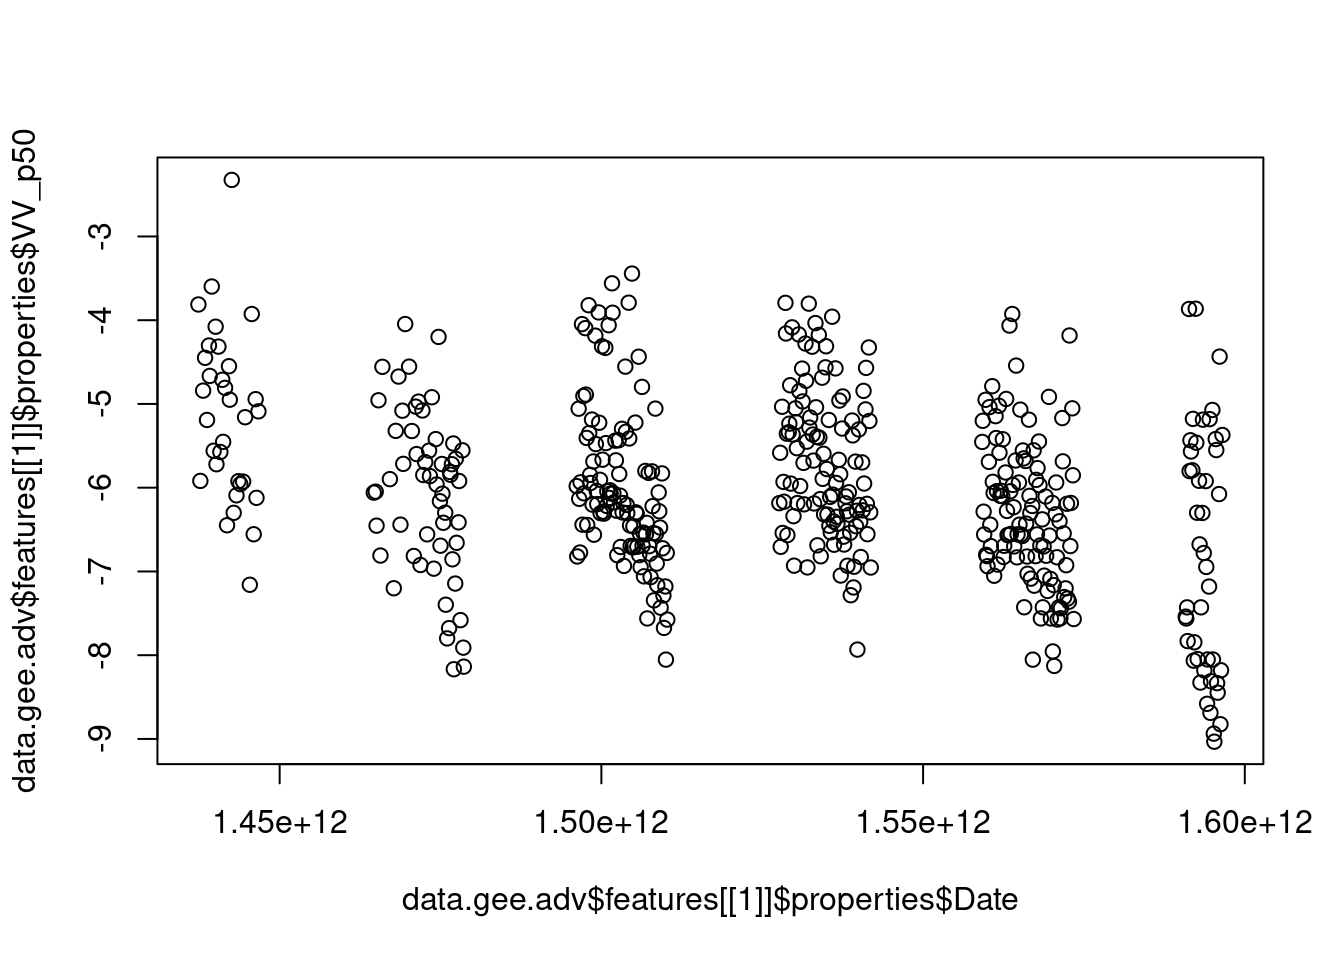
\includegraphics{webinar1_2020_07_29_files/figure-latex/unnamed-chunk-7-1.pdf}
~

~

Then we apply a function to each ``rhomboid'' for creating the square.
It is a bit more complex as the function includes another function
inside.

\begin{Shaded}
\begin{Highlighting}[]
\NormalTok{st_bbox_by_feature =}\StringTok{ }\ControlFlowTok{function}\NormalTok{(geom) \{}
  
  \CommentTok{## make sure that object "geom" becomes a geometry object;}
  \CommentTok{## geom is your data set with all the single geometries/polygons}
\NormalTok{  geom2 =}\StringTok{ }\KeywordTok{st_geometry}\NormalTok{(geom)}
  
  \CommentTok{#' Function to:}
  \CommentTok{#' (a) take a single geometry, }
  \CommentTok{#' (b) create a bounding box with st_bbox and }
  \CommentTok{#' (c) convert the bbox object to a new geometry (a square)}
\NormalTok{  f <-}\StringTok{ }\ControlFlowTok{function}\NormalTok{(single.geom) \{ }
    \KeywordTok{st_as_sfc}\NormalTok{( }\KeywordTok{st_bbox}\NormalTok{(single.geom,), }\DataTypeTok{crs=}\NormalTok{myproj)}
\NormalTok{  \}}
  
  \CommentTok{#' This line calls the function above LOOPING over each single geometry (lapply)}
  \CommentTok{#'  in the geom2 object }
  \KeywordTok{do.call}\NormalTok{(}\StringTok{"c"}\NormalTok{, }\KeywordTok{lapply}\NormalTok{(geom2, f))}
\NormalTok{\}}
\end{Highlighting}
\end{Shaded}

This line calls the above function over our data (rhomboids)

\begin{Shaded}
\begin{Highlighting}[]
\NormalTok{tiles <-}\StringTok{ }\KeywordTok{st_bbox_by_feature}\NormalTok{( nodes.buffered )}
\end{Highlighting}
\end{Shaded}

~

Assign the CRS to the new dataset as it got lost. To check the CRS of
our data we can use \texttt{\{r\}\ st\_crs(tiles)}

\begin{Shaded}
\begin{Highlighting}[]
\NormalTok{tiles <-}\StringTok{ }\NormalTok{tiles }\OperatorTok\StringTok{ }\KeywordTok{st_set_crs}\NormalTok{(myproj) }
\end{Highlighting}
\end{Shaded}

~

We view all results all over the same map (small subset of data - the
first 20 features).

PS you might notice a mis-alignment of the geometries, this is due to
the webgis using a CRS called ``earth universal transverse mercator''
projection which as small deformations when representing data that is in
other CRS.

For more reading see
\href{https://en.wikipedia.org/wiki/Mercator_projection}{Wikipedia}.

\begin{Shaded}
\begin{Highlighting}[]
\KeywordTok{mapview}\NormalTok{( grid.points.myproj[}\DecValTok{1}\OperatorTok{:}\DecValTok{5}\NormalTok{,], }\DataTypeTok{legend =}\NormalTok{ F ) }\OperatorTok{+}\StringTok{ }\KeywordTok{mapview}\NormalTok{( nodes.buffered[}\DecValTok{1}\OperatorTok{:}\DecValTok{5}\NormalTok{,], }\DataTypeTok{legend =}\NormalTok{ F  )  }\OperatorTok{+}\StringTok{ }\KeywordTok{mapview}\NormalTok{( tiles[}\DecValTok{1}\OperatorTok{:}\DecValTok{5}\NormalTok{,], }\DataTypeTok{legend =}\NormalTok{ F  )}
\end{Highlighting}
\end{Shaded}

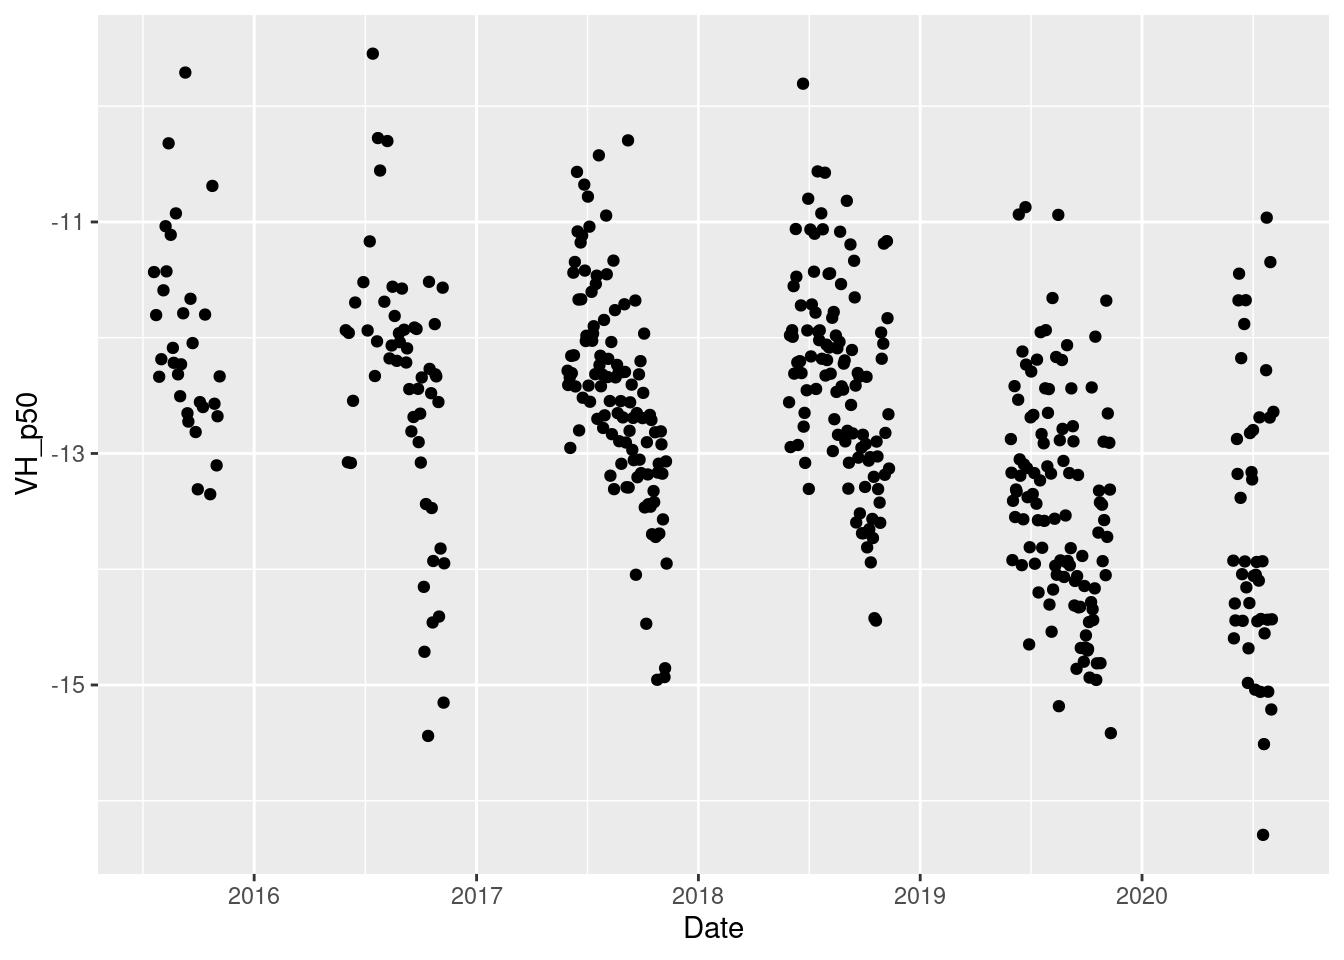
\includegraphics{webinar1_2020_07_29_files/figure-latex/unnamed-chunk-11-1.pdf}

~

\hypertarget{save-result}{%
\subsection{Save result}\label{save-result}}

Convert to Latitude and Longitude and save result to shapefile for
future upload to Google Earth Engine

\begin{Shaded}
\begin{Highlighting}[]
\NormalTok{tiles.latlng <-}\StringTok{ }\NormalTok{tiles }\OperatorTok\StringTok{ }\KeywordTok{st_transform}\NormalTok{(}\StringTok{"+init=epsg:4326"}\NormalTok{)}
\KeywordTok{st_write}\NormalTok{(tiles.latlng, }\StringTok{"data/tiles.shp"}\NormalTok{ )}
\end{Highlighting}
\end{Shaded}

\hypertarget{google-earth-engine-gee}{%
\section{GOOGLE EARTH ENGINE (GEE)}\label{google-earth-engine-gee}}

Import shapefile files ``tiles.XXX'' by left panel ``assets'' and click
``NEW'' and choose shapefile from dropdown menu.

\textbf{DO THINGS in GEE}

code shared: {[}click HERE to open your GEE code editor{]} but also
reported here below

\begin{Shaded}
\begin{Highlighting}[]
\CommentTok{// IMPORTS }
\CommentTok{// these are in the "import" top part of the script editor in GEE, }
\CommentTok{// but can also be added to the script itself.}

\KeywordTok{var}\NormalTok{ srtm }\OperatorTok{=} \VariableTok{ee}\NormalTok{.}\AttributeTok{Image}\NormalTok{(}\StringTok{"CGIAR/SRTM90_V4"}\NormalTok{)}\OperatorTok{;}

\KeywordTok{var}\NormalTok{  srtm_viz }\OperatorTok{=} \OperatorTok{\{}\StringTok{"opacity"}\OperatorTok{:}\DecValTok{1}\OperatorTok{,}\StringTok{"bands"}\OperatorTok{:}\NormalTok{[}\StringTok{"elevation"}\NormalTok{]}\OperatorTok{,}
      \StringTok{"min"}\OperatorTok{:}\FloatTok{1439.9060309998727}\OperatorTok{,}\StringTok{"max"}\OperatorTok{:}\FloatTok{2892.700269813135}\OperatorTok{,}
      \StringTok{"palette"}\OperatorTok{:}\NormalTok{[}\StringTok{"005aff"}\OperatorTok{,}\StringTok{"ff0000"}\NormalTok{]}\OperatorTok{\};} 

\KeywordTok{var}\NormalTok{ tiles }\OperatorTok{=} \VariableTok{ee}\NormalTok{.}\AttributeTok{FeatureCollection}\NormalTok{(}\StringTok{"users/2020_Kanan/summer_webinar_series/Webinar1_tiles"}\NormalTok{)}\OperatorTok{;}


\CommentTok{////////////////////////////////////////////////////////////////////////////////////////////}
\CommentTok{///////////////// PART OF SUMMER WEBINAR SERIES 2020 /////////////////////////////////////// }
\CommentTok{////////////////////////////////////////////////////////////////////////////////////////////}
\CommentTok{/////  Francesco Pirotti - CIRGEO / TESAF Department University of Padova //////////////////}
\CommentTok{////////////////////////////////////////////////////////////////////////////////////////////}
\CommentTok{/////  https://www.cirgeo.unipd.it/shared/R/webinars/webinar1_2020_07_29.html  /////////////}
\CommentTok{////////////////////////////////////////////////////////////////////////////////////////////}
\CommentTok{////////////////////////////////////////////////////////////////////////////////////////////}

 

\CommentTok{// "run" this script and then go to "tasks" button in the right panel to }
\CommentTok{// run also the export of the data. }
\CommentTok{// The last function in this script, "Export...", }
\CommentTok{// will create a "task" that you have to launch manually }
\CommentTok{// to put the final data  to your google drive}


\CommentTok{// this prints info on the "srtm" dataset that we imported }
\AttributeTok{print}\NormalTok{(srtm)}
\CommentTok{// PS double click in the link "SRTM Digital Elevation Data Version 4." above in the}
\CommentTok{// "imports" to see what data we are reading and aggregating at tiles }
\CommentTok{///////////////////////////////////////////////////////////////////////////////////////}

\CommentTok{// this prints info on the "tiles" dataset that we imported from the }
\CommentTok{// shapefile created with R}
\AttributeTok{print}\NormalTok{(tiles)}\OperatorTok{;}
\CommentTok{///////////////////////////////////////////////////////////////////////////////////////}

\CommentTok{// this function below applies the "reduceRegions" function to the "srtm" dataset (image)}
\CommentTok{// over each feature (square polygon in our "tiles" dataset) ... }
\CommentTok{// NB the "reducer" function applies 5 percentiles (10, 25, 50, 75, 90) thus allowing a good}
\CommentTok{// representation of distribution of height values inside the square. }
\CommentTok{// We could also use average and standard deviation as reducers.}
\KeywordTok{var}\NormalTok{  height }\OperatorTok{=}  \VariableTok{srtm}\NormalTok{.}\AttributeTok{reduceRegions}\NormalTok{(}\OperatorTok{\{}
  \DataTypeTok{reducer}\OperatorTok{:} \VariableTok{ee}\NormalTok{.}\VariableTok{Reducer}\NormalTok{.}\AttributeTok{percentile}\NormalTok{([}\DecValTok{10}\OperatorTok{,}\DecValTok{25}\OperatorTok{,}\DecValTok{50}\OperatorTok{,}\DecValTok{75}\OperatorTok{,}\DecValTok{90}\NormalTok{])}\OperatorTok{,} 
  \CommentTok{//reducer: ee.Reducer.mean(), }
  \DataTypeTok{collection}\OperatorTok{:}\NormalTok{ tiles }
\OperatorTok{\}}\NormalTok{)}\OperatorTok{;} 

\CommentTok{// this prints result}
\AttributeTok{print}\NormalTok{(height)}\OperatorTok{;}

\CommentTok{// here we zoom to our tiles and add the layers}
\VariableTok{Map}\NormalTok{.}\AttributeTok{centerObject}\NormalTok{(tiles}\OperatorTok{,} \DecValTok{12}\NormalTok{)}
\VariableTok{Map}\NormalTok{.}\AttributeTok{addLayer}\NormalTok{(srtm}\OperatorTok{,}\NormalTok{ srtm_viz}\OperatorTok{,} \StringTok{"SRTM"}\NormalTok{)}\OperatorTok{;}
\VariableTok{Map}\NormalTok{.}\AttributeTok{addLayer}\NormalTok{(tiles}\OperatorTok{,} \OperatorTok{\{\},} \StringTok{"TILES"}\NormalTok{)}\OperatorTok{;}

\CommentTok{// this exports the data to our Google drive}
 \VariableTok{Export}\NormalTok{.}\VariableTok{table}\NormalTok{.}\AttributeTok{toDrive}\NormalTok{(}\OperatorTok{\{}
    \DataTypeTok{collection}\OperatorTok{:}\NormalTok{ height}\OperatorTok{,}
    \DataTypeTok{description}\OperatorTok{:}\StringTok{'tiles_withData'}\OperatorTok{,}
    \DataTypeTok{fileFormat}\OperatorTok{:} \StringTok{'SHP'}
  \OperatorTok{\}}\NormalTok{)}\OperatorTok{;}
\end{Highlighting}
\end{Shaded}

\textbf{EXPORT THE RESULTS TO A SHAPEFILE CALLED tiles\_withData.shp}

Read the file exported from GEE

\begin{Shaded}
\begin{Highlighting}[]
\NormalTok{grid.points.gee <-}\StringTok{ }\KeywordTok{st_read}\NormalTok{( }\StringTok{"data/webinar1_2020_07_29/tiles_withData.shp"}\NormalTok{ )}
\end{Highlighting}
\end{Shaded}

\begin{verbatim}
## Reading layer `tiles_withData' from data source `/archivio/R/shared/webinars/data/webinar1_2020_07_29/tiles_withData.shp' using driver `ESRI Shapefile'
## Simple feature collection with 1315 features and 6 fields
## geometry type:  POLYGON
## dimension:      XY
## bbox:           xmin: 11.82833 ymin: 46.32735 xmax: 12.14759 ymax: 46.55912
## geographic CRS: WGS 84
\end{verbatim}

\hypertarget{r---plot}{%
\section{R - Plot}\label{r---plot}}

\hypertarget{calculate-new-iqr-field}{%
\subsection{Calculate new IQR field}\label{calculate-new-iqr-field}}

Create a new attribute column with the interquartile range (The
difference between p75 and p25, i.e.~75th and 25th percentile)

\begin{Shaded}
\begin{Highlighting}[]
\NormalTok{grid.points.gee}\OperatorTok{$}\NormalTok{iqr<-grid.points.gee}\OperatorTok{$}\NormalTok{p75 }\OperatorTok{-}\StringTok{ }\NormalTok{grid.points.gee}\OperatorTok{$}\NormalTok{p25}
\end{Highlighting}
\end{Shaded}

\newpage

\hypertarget{plot-variables}{%
\subsection{PLOT variables}\label{plot-variables}}

\begin{Shaded}
\begin{Highlighting}[]
\NormalTok{pal =}\StringTok{ }\KeywordTok{mapviewPalette}\NormalTok{(}\StringTok{"mapviewSpectralColors"}\NormalTok{)}
\KeywordTok{mapview}\NormalTok{( grid.points.gee, }\DataTypeTok{col.regions =} \KeywordTok{pal}\NormalTok{(}\DecValTok{100}\NormalTok{), }\DataTypeTok{zcol =} \StringTok{"p50"}\NormalTok{, }
         \DataTypeTok{color=}\OtherTok{NULL}\NormalTok{, }\DataTypeTok{alpha.regions=}\FloatTok{0.8}\NormalTok{  ) }
\end{Highlighting}
\end{Shaded}

\includegraphics{webinar1_2020_07_29_files/figure-latex/unnamed-chunk-16-1.pdf}
Figure 1 - 50th Percentile (median)

\newpage

\begin{Shaded}
\begin{Highlighting}[]
\KeywordTok{mapview}\NormalTok{( grid.points.gee, }\DataTypeTok{col.regions =} \KeywordTok{pal}\NormalTok{(}\DecValTok{100}\NormalTok{), }\DataTypeTok{zcol =} \StringTok{"p10"}\NormalTok{, }
         \DataTypeTok{color=}\OtherTok{NULL}\NormalTok{, }\DataTypeTok{alpha.regions=}\FloatTok{0.8}\NormalTok{  ) }
\end{Highlighting}
\end{Shaded}

\includegraphics{webinar1_2020_07_29_files/figure-latex/unnamed-chunk-17-1.pdf}
Figure 2 - 10th Percentile

\newpage

\begin{Shaded}
\begin{Highlighting}[]
\KeywordTok{mapview}\NormalTok{( grid.points.gee, }\DataTypeTok{col.regions =} \KeywordTok{pal}\NormalTok{(}\DecValTok{100}\NormalTok{), }\DataTypeTok{zcol =} \StringTok{"iqr"}\NormalTok{, }
         \DataTypeTok{color=}\OtherTok{NULL}\NormalTok{, }\DataTypeTok{alpha.regions=}\FloatTok{0.8}\NormalTok{)}
\end{Highlighting}
\end{Shaded}

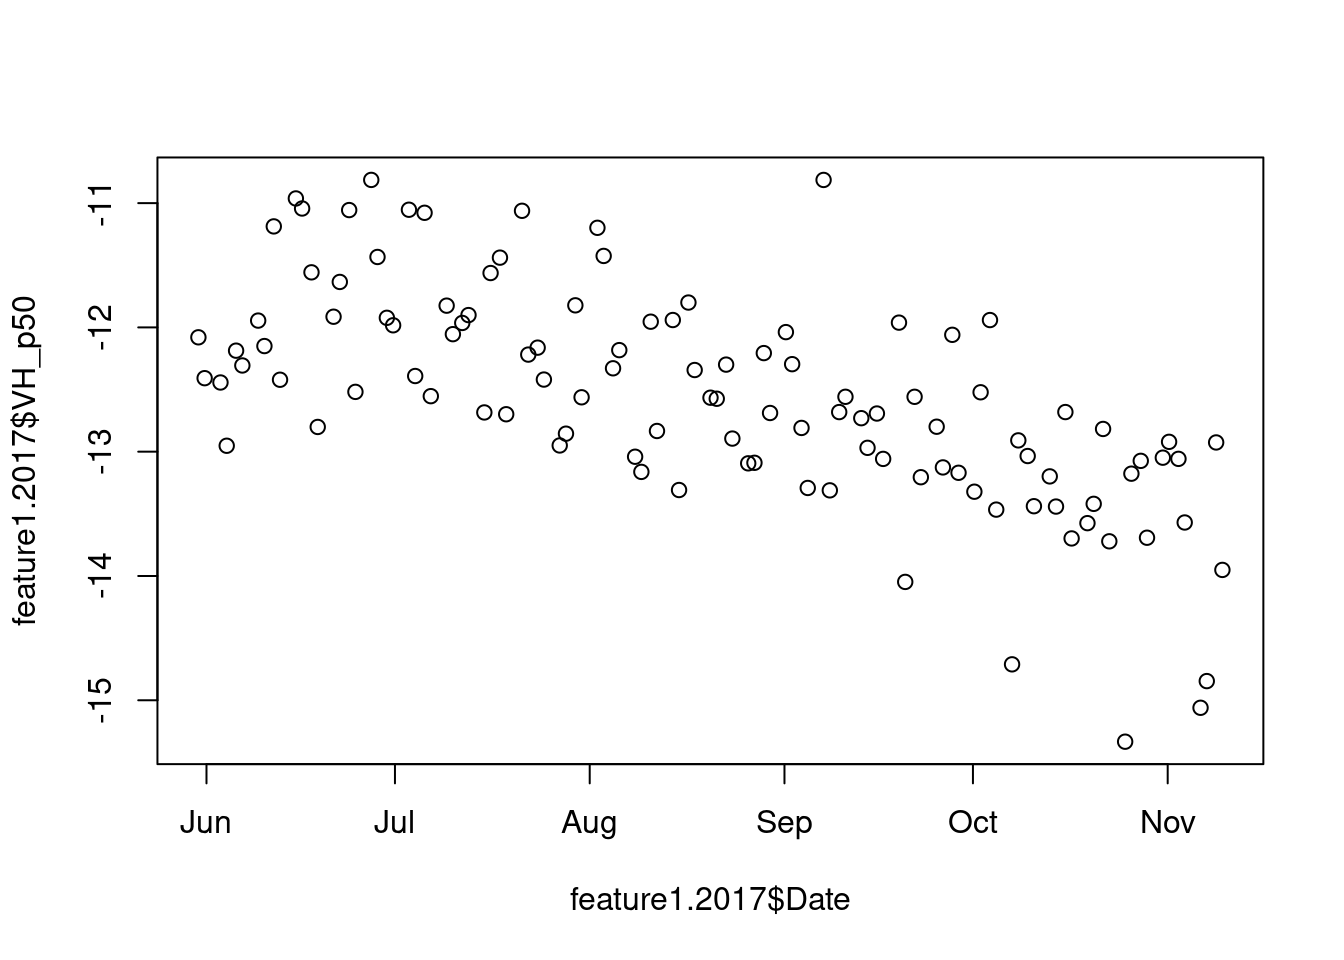
\includegraphics{webinar1_2020_07_29_files/figure-latex/unnamed-chunk-18-1.pdf}
Figure 3 - Inter Quartile Range

\begin{Shaded}
\begin{Highlighting}[]
\KeywordTok{sessionInfo}\NormalTok{()}
\end{Highlighting}
\end{Shaded}

\begin{verbatim}
## R version 3.6.3 (2020-02-29)
## Platform: x86_64-pc-linux-gnu (64-bit)
## Running under: Ubuntu 20.04.1 LTS
## 
## Matrix products: default
## BLAS:   /usr/lib/x86_64-linux-gnu/atlas/libblas.so.3.10.3
## LAPACK: /usr/lib/x86_64-linux-gnu/atlas/liblapack.so.3.10.3
## 
## locale:
##  [1] LC_CTYPE=en_US.UTF-8       LC_NUMERIC=C              
##  [3] LC_TIME=en_US.UTF-8        LC_COLLATE=en_US.UTF-8    
##  [5] LC_MONETARY=en_US.UTF-8    LC_MESSAGES=en_US.UTF-8   
##  [7] LC_PAPER=en_US.UTF-8       LC_NAME=C                 
##  [9] LC_ADDRESS=C               LC_TELEPHONE=C            
## [11] LC_MEASUREMENT=en_US.UTF-8 LC_IDENTIFICATION=C       
## 
## attached base packages:
## [1] stats     graphics  grDevices utils     datasets  methods   base     
## 
## other attached packages:
## [1] raster_3.0-7  sp_1.4-1      mapview_2.7.8 sf_0.9-5     
## 
## loaded via a namespace (and not attached):
##  [1] tidyselect_0.2.5   xfun_0.10          purrr_0.3.3       
##  [4] lattice_0.20-40    colorspace_1.4-1   viridisLite_0.3.0 
##  [7] htmltools_0.4.0    stats4_3.6.3       yaml_2.2.0        
## [10] base64enc_0.1-3    rlang_0.4.5        leafpop_0.0.1     
## [13] e1071_1.7-2        later_1.0.0        pillar_1.4.2      
## [16] glue_1.3.1         DBI_1.1.0          stringr_1.4.0     
## [19] munsell_0.5.0      htmlwidgets_1.5    codetools_0.2-16  
## [22] evaluate_0.14      knitr_1.25         callr_3.3.2       
## [25] fastmap_1.0.1      ps_1.3.0           httpuv_1.5.2      
## [28] crosstalk_1.0.0    class_7.3-15       leafem_0.1.1      
## [31] Rcpp_1.0.3         KernSmooth_2.23-16 xtable_1.8-4      
## [34] promises_1.1.0     scales_1.0.0       classInt_0.4-1    
## [37] satellite_1.0.1    jsonlite_1.6       webshot_0.5.1     
## [40] leaflet_2.0.2      mime_0.7           png_0.1-7         
## [43] digest_0.6.21      stringi_1.4.6      processx_3.4.2    
## [46] dplyr_0.8.5        shiny_1.4.0        grid_3.6.3        
## [49] tools_3.6.3        magrittr_1.5       tibble_2.1.3      
## [52] crayon_1.3.4       pkgconfig_2.0.3    assertthat_0.2.1  
## [55] rmarkdown_2.2      R6_2.4.1           units_0.6-4       
## [58] compiler_3.6.3
\end{verbatim}

\end{document}
